\Chapter{Témaköri felvezetés}

\Section{A póker alapjai}
Ahhoz, hogy a szakdolgozat értelmet kapjon, mindenképp tisztázni kell néhány, a pókerrel kapcsolatos alapfogalmat, valamint a játék menetét. Ebben a szakaszban ezekről fogok írni.

\subsection{A játék menetének kifejtése}
A játék menetét illetően próbálok csak a számunkra releváns részletekre koncentrálni. Egy játék sok leosztásból áll, attól függ milyen típust játszunk. A játékosok száma is eltérő, általában 5 és 10 közötti látszámmal szokták játszani. Minden játékosnak kezdetben egyenlő összegű zsetonkészlete van, amivel játszhat. Mindig van egy osztó, akit az első leosztásnál solrsolnak, a tőle bal oldalon ülő játékos a kis vak, az osztótól balra a második játékos pedig a nagy vak. Ha van kijelölt osztó az asztalnál, akkor egy gombbal jelzik, ki birtokolja az osztó pozíciót, ez a gomb megy körbe. A játékot az óramutató járásával megyegyező irányban játszák. % egy helyesírásellenőrzést majd eresz rá, van benne pár elgépelés 

Amint be van rakva a kisvak és a nagy vak, kezdődhet a játék. Az osztó a kis vaknak oszt előszőr egy lapot, majd körbe mindenkinek, ezután megint egy lapot mindenkinek. A beszédet a nagy vak mellett ülő játékos kezdheti, vagyis ő nyilatkozhat először lapjairól. Alapvetően három választási lehetősége van, ahogy mindenkinek az asztalnál. Bedobja lapjait, beszáll, vagyis megadja az alaptétet, vagy pedig emel. Miután mindenki beszélt az asztalnál (utoljára a nagy vak),% nem pontos, miután az utolsó licitkör lement 
 akkor az osztó egy lapot éget, vagyis letesz az asztalra fejjel lefelé, ami már nincs játékban. Ez után három lapot kirak egymás után, hogy mindenki lássa. Itt jön a második licitkör. Ebben az esetben már a kis vak kezdi a beszélést. Ugyan az a három lehetősége van, majd ha mindenki beszélt (az osztó utoljára), % nem pontos, miután az utolsó licitkör lement 
  akkor még egy lap égetése, majd immáron csak egy lap asztalra helyezése következik. Megint jön egy licitkör, majd még egy égetés, és az utolsó felfordított lap az asztalra. Maradt még egy utolsó licitkör, és elérkeztünk a játék végéhez.

Abban az esetben nyer valaki, ha a bentmaradt játékosok közül neki van a legerősebb lapja, vagy ha nem maradt más játékban csak egy valaki. A lent lévő 5 lapból és a kezünkben lévő 2-ből, összesen 5-öt választhatunk ki, így alakul ki a kezünk. Ezzel lement egy parti a játékból. Valakinek gyarapodott a zsetonkészlete, valakinek csökkent. % jobb esetben. Lehet nincs változás.

\begin{figure}[h]
\centering
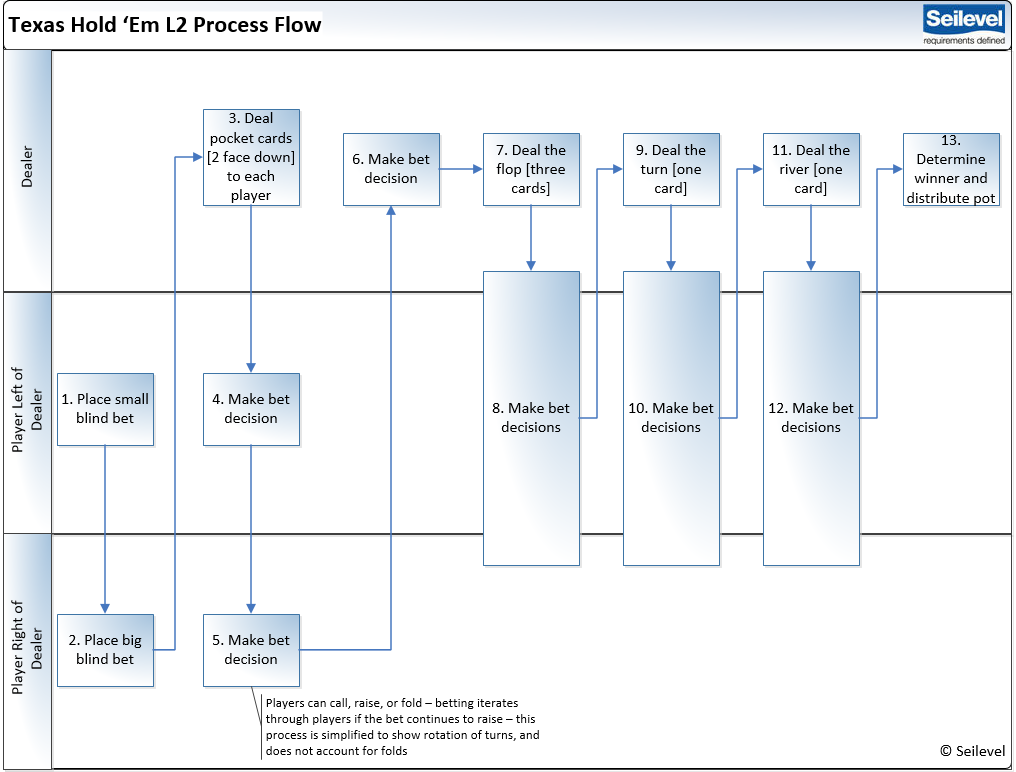
\includegraphics[scale=0.4]{images/process-flow.png}
\caption{Folyamatábra a póker menetéről}
\cite{process-flow}
\label{fig:process-flow}
\end{figure}

\subsection{Alapfogalmak}
Elengedhetetlen, hogy tisztázzunk néhány alapfogalmat. Ezek a következők.
\cite{harrington}
\begin{itemize}
\item Flop: Három kártyalap, ami egyszerre kerül az asztalra, színével fölfelé. Ezek a lapok a játékosok közös lapjai. A flop után egy újabb licitkör következik.
\item Gomb vagy osztó (Button): A kis vak jobb oldalán ülő játékos. A flop után ő kerül utoljára sorra minden licitkörben. A gombot egy fehér korong jelzi, ami az óramutató járásával megegyező irányban körbejár az asztalon.
\item Jó (Out): Olyan lap(ok), mellyek kezünk nyerővé alakulna.
\item Kezdeti bank (Initial pot): A vaktét és az esetleges alaptétek összege a licitálás megkezdése előtt.
\item Kis vaktét (Small blind): Az osztó bal oldalán ölő játékos által a licitsorozat megkezdéseként kötelezően betett tét.
\item Nagy vaktét (Big blins): A kis vak bal oldalán ölő játékos által kötelezően betett tét, a további akciók motiválására.
\item Turn: A negyedik közös lap, ami színével fölfelé az asztal közepére kerül. A turn után újabb licitkör következik.
\item River: Az ötödik és egyben utolsó közös lap, ami az asztal közepére kerül színével fölfelé. A river után az utolsó licitkör következik.
\item Saját lapok (Hole cards): Az egyes játékosoknak a parti elején színével lefelé kiosztott két-két kártyalap. Ezeket a lapokat a többi játékos nem láthatja.
\item Kéz: Egy játékos által, a lent lévő és a kezében lévő lapok közül kiválasztott öt lap.
\item Nuts: A lehető legjobb kombinációval rendelkező játékos keze.
\item Zsetonkészlet (Stack): Egy adott játékos előtt az asztalon lévő zsetonmennyiség.
\end{itemize}

\subsection{Piackutatás}
Mielőtt belekezdtem volna az alkalmazás elkészítésébe, végeztem egy kis piackutatást, milyen platformok/programok vannak, amik a témával foglalkoznak.

Nem kellett messzire mennem, hogy az elsőre rábukkanjak, hiszem a póker közvetítéseken láthatjuk, hogy ki van írva a játékosok nyerési esélye, egy-egy leosztásnál. Ott viszont a program ismeri a játékban lévő játékosok lapjait, valamint az asztalon lévő lapokat. Így könnyebb meghatározni melyik játékos nyer, vagy legalábbis kevesebb számítást igényel. Esetemben az alkalmazás csak a saját lapomat, valamint az asztalon lévőket ismeri.

Létezik egy technika a témával kapcsolatban, amivel a profi póker játékosok az esélyeiket számolják. A lényege csupán annyi, hogy kiszámolják a lehetséges out-okat, amivel javul a kezük, ezeket megszorozzák kettővel, majd annyival, ahány lapra még várunk. Flop esetén kettővel, turn esetén egyel. Így kapnak egy számot, ami ha nagyobb, mint a banki esélyük, akkor matematikailag, vagy éppen gazdaságilag kifizetődő tartani a tétet. Ezzel a megoldással szemben az én elképzelésem alapján nem csak egy közelítő értéket fogunk kapni, hanem specifikusan minden lehetséges leosztásra egy pontos értéket kapunk, emellett még más adatokat is, melyek segítenek eldönteni a felhasználónak mi legyen a következő lépés.

Az interneten két hasonló programot találtam a póker esélyek számítására, mindkettő webalkalmazás és külalakra hasonlítanak az én elképzelésemre. Az elsőnél csak úgy lehet használni az alkalmazást, ha legalább két játékosnak megadjuk a lapjait. Ezzel a probléma ugyan csak az, mint a fent említett televíziós közvetítéseknél ismert megoldással. Ezt az alkalmazást a chardchat.com weboldalon találtam, ami a világ elsőszámú pókeres online közössége.

\begin{figure}[h!]
\centering
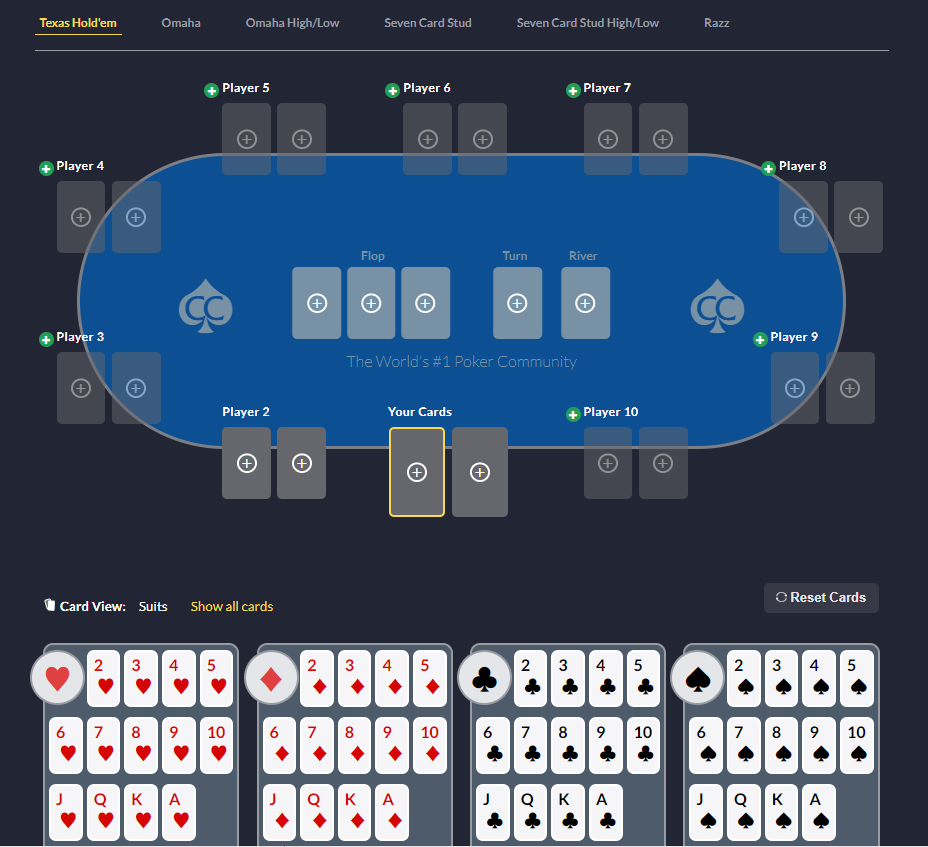
\includegraphics[scale=0.6]{images/cardschat.png}
\caption{Cardschat Poker Odds Calculator}
\label{fig:cardschat}
\end{figure}

A másik szoftver, ami talán a legjobban megközelíti a megoldásomat, a pokernews.com oldalán lévő webalkalmazás. Érdekesség, hogy ezt szintúgy egy óriás, pókerrel foglalkozó cég szponzorálta. A világ talán leghíresebb online póker platformja, a legnagyobb póker versenyek rendezője, a PokerStars. Ebben az esetben tudunk esélyeket számolni úgy is, hogy csak egy játékost választunk ki, csak úgy, mint az én megoldásomnál. Le tudunk rakni 1 és 9 között tetszőleges számú játékosokat, az alkalmazás pedig ezt figyelembe véve számolja az esélyeket. Ezen felül még további esélyeket is látunk, hogy hány százalék a valószínűsége annak, hogy párunk, drillünk, pókerünk, stb. alakuljon ki. Ez a megoldás nagy részben lefedi az általám kigondolt megvalósítást. A különbség, hogy én csak azt szeretném látni, hogy mennyi az esélyem a nyerésre. Az, hogy különböző kezek milyen esélyben alakulnak ki, számomra lényegtelen. Ezzel szemben olyan matematikai mutatók, mint az átlag, a medián vagy a relatív gyakoriság sokkal fontosabb tudni, hogy segítsen a felhasználónak bemutatni az esélyeit.
\begin{figure}[h!]
\centering
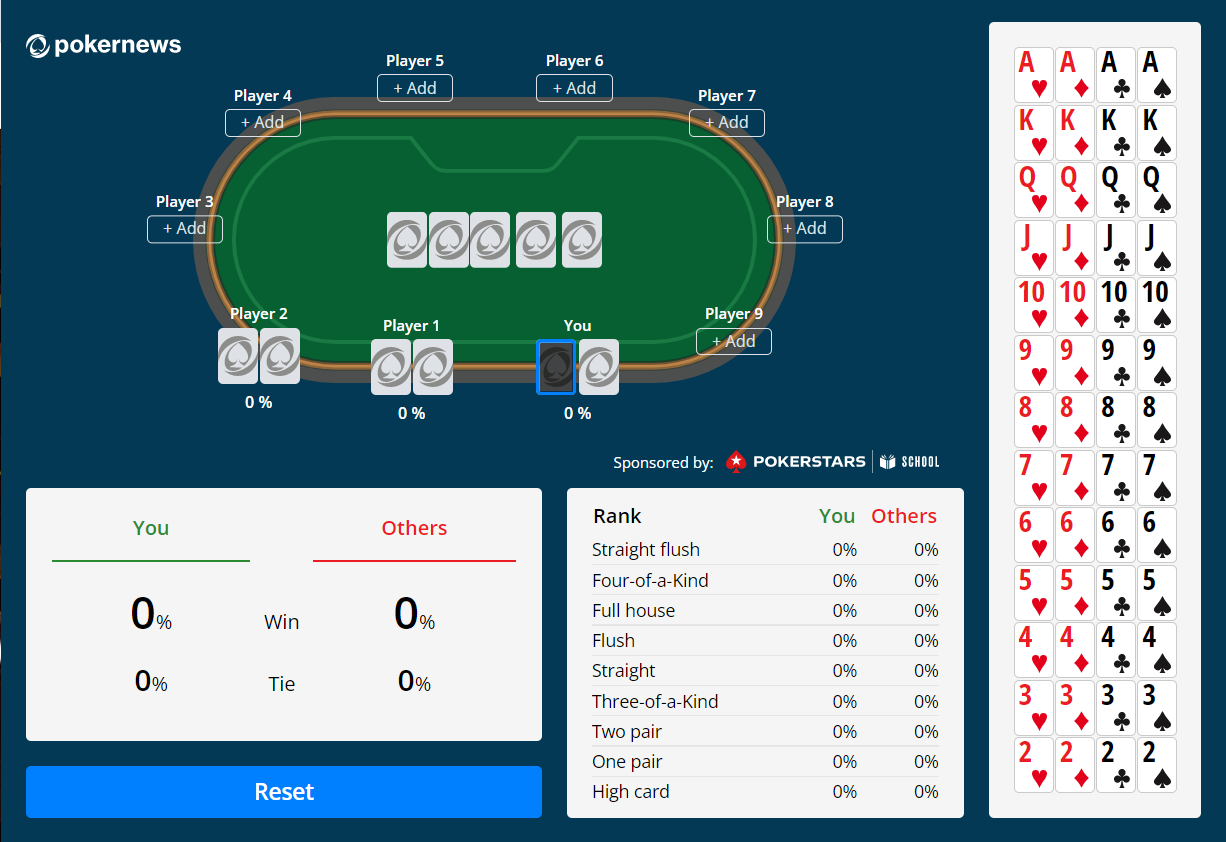
\includegraphics[scale=0.5]{images/pokerstars.png}
\caption{Pokerstars Texas Hold'Em Poker Odds Calculator}
\label{fig:pokerstars}
\end{figure}

\cite{cardschat}
\cite{pokerstars}
\cite{harrington} %hivatkozások mehetnek az utolsó mondat még. Ne álljanak külön 

\Section{Felhasznált technológiák}
Ebben a szakaszban bemutatom az összes olyan technológiát, programozási nyelvet, keretrendszert vagy könyvtárat, amit felhasználtan a szakdolgozatom elkészítése során. Törekszem a tömör magyarázatra. Mindegyiknél próbálom elmagyarázni miért választottam, valamint mik az előnyei, amik számomra kedvezőek voltak.

\subsection{Egyoldalas webalkalmazások}

Ha figyelemmel követjük a Javascript keretrendszerek fejlődését, akkor láthatjuk, hogy egyre nagyobb teret kapnak az egyoldalas alkalmazások (Single Page Application), az olyan többoldalas alkalmazásokkal (Multi Page Application) szemben, mint a jQuery vagy a Laravel.

Három elterjedt Javascript keretrendszert különböztetünk meg. A Facebook által fejlesztett React-ot, az Angulart, amit a Google hozott létre és az Evan You alkotott Vue JS-t.
\cite{vue}

\subsection{Vue JS}

Mindhárom SPA-nak megvan a maga előnye és hátránya. Ezek közül inkább csak a Vue előnyeire koncentrálok a másik kettővel szemben. A három közül ez a legkönnyebben tanulható. Használatához nem szükséges különösebb meglévő Javascript tudás, enélkül is könnyen el lehet sajátítani.

A maga 18 KB-os méretével rendkívül kicsinek számít, amit könnyű letölteni és feltelepíteni, ennek ellenére pozitívan hat a felhasználói élményre és jó keresőmotor optimalizálással is rendelkezik. Saját virtuális DOM-ot (Document Object Model) renderel, ami jobban teljesít mint a React vagy az Angular. Könnyen olvasható a kódja, könnyen integrálható, jól dokumentált, és ezen kívül sok más előnye is van.

Többek között a Vue JS egyik fő tulajdonsága - ami megvan a többi SPA-ban is - hogy komponensekből épül fel, amiket újra felhasználhatunk, ezzel is elősegíti a rövidebb programkódot, átláthatóságot, egyszerűséget, amiket már fent említettem.

Ezek miatt esett a választásom a Vue JS-re, amire több forrás keretrendszerként, mások pedig könyvtárként hivatkoznak
\cite{vue}. %hivatkozást a mondatba rakunk. Ott ahol hivatkoztunk rá. lásd előző mondtat. 

\subsection{Node JS és az Express}

Amellett, hogy a legnépszerűbb programozási nyelv, a Javascript az egyik leginkább univerzális szoftverfejlesztési technológia. Hagyományosan frontend fejlesztésre használták, viszont az utóbbi időben elterjedt a szerver oldali (backend) használata is. Az egyik eszköz - és talán a legismertebb - ami ezt az elmozdulást elősegítette az a Node JS.

A Node JS tulajdonképpen nem egy keretrendszer, nem is egy könyvtár, hanem egy futtató környezet, ami a Chrome V8-as motorján alapszik. A technológiát először 2009-ben mutata be Ryan Dahl az Európai Javascript Konferencián. Amellett, hogy ezen a konferencián rögtön elnyerte a legizgalmasabb szoftver díjat, nem volt használatos széles körben. A technológia 2017-ben csúcsosodott ki, amikor is először használta egy ismertebb cég, a LinkedIn, vagy, hogy még egy párat említsek, a Netflix, eBay és az Uber.

Az egyik hatalmas előnye a Node JS használatának, hogy autómatikusan teljeskörű (full stack) web fejlesztővé válunk vele. Gondoljunk csak bele, két legyet ütünk egy csapásra. Egyszerűen nincs alternatívája a szerver oldali programozásnak a Javascript-ben, csak a Node JS, ez teszi megkerülhetetlenné a technológiát.

Ezek mellett gyors feldolgozású, mivel közös nyelvet használ a frontend és a backend, így a szinkronizáció gyors. Esemény alapú modell-t (event-based model) használ, ezért népszerű választás online játékok, vagy videó konferenciák készítéséhez. Gazdag az ökoszisztémája, az npm - ami a Node JS alapértelmezett csomagkezelője - paranccsal több, mint 800 ezer könyvtárat érhetünk el. Ezen felül több, számos előnye is van, amikre nem térek ki.

Az Express a legnépszerőbb Node JS keretrendszer. Köztes szoftverként (middleware) hivatkoznak rá, amely annyit tesz, hogy tulajdonképpen a kliens és a szerver oldal közötti híd felépítéséhez biztosít eszközöket. Könnyű, rugalmas és véleménymentes keretrendszer. Véleménymentes, mert semmilyen módon nem korlátozza a fejlesztőt, így nagy szabadságot ad. Emellett nagy teljesítményű és hatalmas közössége van a sok felhasználó miatt.
\cite{node}

\subsection{Chart JS}
A Chart JS egy nyílt forráskódú javascript könyvtár adatok megjelenítésére, amely nyolc féle diagramm típust támogat. 2013-ban fejlesztették, mára a második legnépszerűbb diagram készítő javascript könyvtár a GitHub-on. Meglepően egyszerű használni, ez volt a fő oka, amiért ezt választottam. 

A Chart JS HTML5-be renderel. Az én célomhoz csupán két féle diagram típust kell használnom. Az oszlopdiagramot és a vonaldiagramot, ezeket kell egybefűznöm és úgy megjelenítenem.
\cite{chartjs}

\subsection{HTML}
A HTML-ről (Hypertext Markup Language) nem szeretnék hosszasan írni. Talán egy laikus is tudja, hogy ha webalkalmazásról van szó, vagy akár csak egy honlapról, akkor megkerülhetetlen a HTML.

A HTML-t weboldalak készítésére hozták létre, amit később bárki elérhet, aki rendelkezik internet kapcsolattal (feltéve, hogy fel van töltve a weboldal egy domain-re). Használhatunk benne főcímeket, paragrafusokat, beépített képeket, videókat. Ezeket úgynevezett tag-ek határoznak meg. Az elején a kezdő tag, a végén pedig a záró tag.

Szakdolgozatomban a HTML5-öt használtam, amit 2014-ben mutattak be. Többek között olyan újításokat tartalmazott, mint a beépített audio és video tartalom.
\cite{web}

\subsection{CSS}

A CSS (Cascading Style Sheets) egy stílusleíró nyelv. Alkalmazása a HTML elemek kinézetére irányul, azaz hogyan szeretnénk láttatni a weboldalunkon megjelenő tartalmakat.

A CSS a HTML elemekre hat, a kommunikálás pedig többek között a selector-ok segítségével történik. Ezeket a CSS alapból tartalmazza, hivatkozhatunk egy megformálni kívánt paragrafusra, főcímre, valamint megadhatunk saját osztályokat is, amiket többször fel tudunk használni. A deklaráció tulajdonságokat és értékeket tartalmaz.

Itt szeretnék megemlíteni két dolgot, amit a szakdolgozatom készítése során tapasztaltam. Az egyik, hogy érdekes volt számomra megfigyelni, hogy leginkább ez a rész volt az, ami felkeltette az érdeklődésem, ebben tudtam maximálisan kiteljesedni. A másik pedig, hogy megjegyezném az egyre elterjedtebb felhasználási módját a CSS-nek. Ez pedig nem más, mint a Bootstrap, amit azért hoztak létre, hogy könnyedén készítsünk reszponzív weboldalakat, azaz minden képernyőméreten szépen megjelenő oldalakat.

Esetemben tudtam, hogy az én alkalmazásomat számítógép képernyőjén, esetleg más eszközökön, de kizárólag fektetett állapotban lehet használni. Éppen ezért nem láttam értelmét mélyebben beleásni magam ebbe a világba.
\cite{web}

\subsection{Google Firebase}
A Firebase egy szoftverfejlesztő platform, ami 2011-ben indult és 2014-ben került a Google tulajdonába. Valósidejű adatbázisként (Realtime Database) indult, mostanra viszont 18 szolgáltatása és dedikált API-ja (Application Programming Interface) van. Az egész platform egy úgynevezett Backend-as-a-Service megoldást kínál mobil és webalapú alkalmazásokhoz, amely szolgáltatást tartalmaz az alkalmazások fejlesztésére, tesztelésére és kezelésére. 

Számomra a legfőbb előnyei a technológiának, amiért ezt választottam a következők. Teljesen ingyenesen lehet használni a legtöbb szolgáltatását. Könnyű hozzáférést biztosít az adatokhoz, a Firbease console-on keresztül. Könnyő az integrálása is és minimális programozási ismereteket kíván, tehát majdnem, hogy bárki be tudja építeni az alkalmazásába.

Annak ellenére, hogy ez egy nagyon összetett paltform, az alkalmazásom kizárólag a Real Time Database-t használja ezekből. A Google Firebase végzi az autencikációt, vagyis a regisztrációt és a bejelentkezést az oldalra.
\cite{firebase}

\subsection{JSON}
A JSON (Javascript Object Notation) egy szövegalapú nyílt szabvány, amit emberek számára is könnyen olvasható adatátvitelre terveztek. Javascript alapú alkalmazásokhoz, valamint hálózati kapcsolaton keresztüli továbbításra használják. 

Egyik és talán legfontosabb előnye, hogy a legtöbb script nyelvben közvetlenül megfelel az alapvető adattípusoknak, továbbá különbséget tesz a string, number és boolean értékek között. Tehát könnyedén lehet használni a webfejlesztés során. 

Objektumokat hozhatunk benne létre, melyekre kulcsokkal tudunk hivatkozni. Számomra ez volt a fő szempont, mert nagy adathalmazzal kell dolgoznom és ezekben keresést végezni, ami ezzel a módszerrel gyorsnak tekinthető.

\Section{Tervezés}

\subsection{Az alkalmazás megjelenítése}
Az alapvető elképzelésem az alkalmazás külsejéről az volt, hogy az oldalra érkezéskor rögtön egy autentikációs felület fogadja a felhasználót. Ezzel egy amolyan privát jelleget szerettem volna kölcsönözni az egésznek, hogy csak az használhassa, aki regisztrált. A regisztráció/bejelentkezés után egy főoldal fogad minket. Ezen az oldalon a Texas Hold'Em póker változatról egy rövid leírást mutatok be, valamint az alkalmazás lényegét szemléltetem. Az oldal tetején van egy egyszerű navigácóis felület, ahol tovább mehetünk arra az oldalra, ahol magát a játékot találjuk.

Itt is az egyszrűséget tartom szem előtt. Középen helyezkedik el egy pókerasztal felülnézetből. Alatta jelenítem meg a négy színt (treff, káró, kör, pikk). Ezekre rákattintva előjön az adott színből az összes (13) kártya, ami közül kiválasztunk először egyet, ez a lap pedig eltűnik a választható lehetőségek közül és lekerül az asztalra saját lapként. Megint a négy színt látjuk, amiből ismét kiválasztunk egyet, és még egy lapot. Ezek után ugyan ezzel a módszerrel tudjuk lehelyezni az asztal közepére is a közös lapokat.

Minden licitkör előtt az asztal mellett láthatja a felhasználó az összesített nyerési esélyét, ami segít neki a döntés meghozásában. Ha több lapot szeretne a felhasználó az asztalra tenni mint a 2 (saját) + 5 (közös), akkor egy pop up ablak ugrik fel, ami jelzi neki, hogy már több lapot nem használhat. Két választása van ebben az esetben, az egyik, hogy figyelmen kívül hagyja, ilyenkor elemezheti tovább az esélyeket. A másik, hogy új leosztást kezd, ilyenkor eltűnik minden lap az asztalról és folytathatja a játékot.

\subsection{Alapötlet} % Jól megírtad és átadtad a lényeget. 
A tervezés első lépése a módszer meghatározása volt, amellyel az esélyeket számoljuk. Ezt hátulról előre haladva közelítettem meg, azaz a rivernél kezdtem, a turn-ön át, egészet a preflopig. Ennek oka az volt, hogy a legkevesebb számítás akkor van, amikor minden lap lent van és tudjuk, hogy nekünk milyen erős kezünk van, így azzal ebben az esetben nem kell folglakozni, tehát bonyolultsági sorrendben haladtam.

Az alapötlet az volt, hogy legenerálom az összes lehetséges 7 lap együttesét, amelyekhez egy értéket rendelek, hogy mennyire erősek. Természetesen a legerősebb a royal flush, a leggyengébb pedig a 7-es magaslap. Csak, hogy szemléltessem a számolások bonyolultságát és nagyságát, ez \[ \binom{52}{7}=133.784.560\] eset. Turn esetében ismerem az én 7 lapomat, tehát csak egy keresést kell végezni ebben az adathalmazban, ami visszatér a kezem értékével. Az ellenfél esélyeinek kiszámítása már egy kicsit komplikáltabb. Az 52 lapból ismerünk 7-et, tehát a pakliban 45 lap marad. Ebből választhat további 2 lapot az ellenfél, ez \[ \binom{45}{2}=990\] lehetőség az ellenfél kezeire. Ez a szám fontos szerepet játszik a dolgozat történetében, és végig jelen lesz a dokumentációban. Erre a 990 lehetőségre mind el kell végezni a keresést a kb. 133 milliós adathalmazban, így kapunk 990 értéket. Innentől kezdve már csak az a dolgunk, hogy hány százalékban kissebb a mi kezünk értéke az ellenfél lehetséges kezeinél. 

Tovább haladva a turn esetében vizsgáljuk az esélyeket, amikor is csak 4 lap van az asztalon, egy lapra pedig még várunk, ami egyelőre ismeretlen. Itt kissé bonyolultabb a helyzet, mivel a saját kezünk értékét sem ismerjük. Természetesen vannak szélsőséges esetek, mikor már a turn-nél pókerünk vagy royal flush-ünk alakul ki, ezekben az esetekben nem releváns az utolsó lap, mindenképp nyertünk. Ilyen esetek azonban ritkán fordulnak elő. Először ki kell számolnunk a saját esélyeinket, amit majd össze tudunk hasonlítani az ellenfél esélyeivel. Két lap a kezünkben, négy lap az asztalon, 46 lap maradt, ami érkezhet az asztalra utolsóként. Mind a 46 lapra meg kell keresnünk az adathalmazban a kezünk értékét, így a saját kezeinkre lesz 46 értékünk. Ezután mind a 46 lehetséges utolsó lapra meg kell keresnünk az ellenfél 990 lehetséges kezére az értékeket, ez 45.540 eset. Amint ezek megvannak, össze tudjuk hasonlítani az értékeket.

A flop esetében lévő értékek számításánál még több számítást kell végeznünk. A saját két lapunkon kívül itt már csak három lent lévő lapot ismerünk. Ez azt jelenti, hogy turn-re jöhet 47 féle lap, river-re pedig további 46 féle. A saját lapjaink \[ \binom{47}{2}=1081\] féle képpen jöhetnek le. Ezek alapján az ellenfélnek \[1081\cdot990=1.070.190\] lehetséges keze van. Ezekre a lehetséges kombinációkra mind keresést kell végeznünk az adathalmazban, hogy megkapjuk a saját és az ellenfél értékeit, amivel tovább tudunk dolgozni.

<<<<<<< Updated upstream
Az utolsó licitkör, aminél számításokat kell végeznünk, az tulajdonképpen a játék menetét illetően az első licitkör. A preflop esetben nem ismerünk semmilyen lapot, csak azt a kettőt, amit osztottak nekünk. Az 52 lapos pakliból 50 lap érkezhet az asztalon lévő első helyre, a másodikra 49, az ötödikre, vagyis az utolsóra pedig 46 lehetséges lap. Itt kell a legtöbb számítást végezni, amikor is \[ \binom{50}{5}=2,118,760\] különbözőképpen alakulhat ki a saját kezünk. Ezt megszorozva a már ismert rivern-nél lévő ellenfél kezeinek kombinációjával, az ellenfél lehetséges kezeinek száma 2.097.572.400, ami több, mint két milliárd eset. Ennyi értékkel kell majd számolnunk a továbbiakban. Ez jól mutatja, hogy milyen összetett a problémakör és, hogy mennyi számítást igényel. Az alapötletben ezt nem számoljuk valós időben, hiszen rengeteg időt venne igénybe. Ehelyett egyszer legeneráljuk ezeket a kombinációkat az összes lehetséges kézre preflop, ami 1326 lehetőség, tehát ennyivel kell megszoroznunk még a fent említett számot.
=======
Az utolsó licitkör, aminél számításokat kell végeznünk, az tulajdonképpen a játék menetét illetően az első licitkör. A preflop esetben nem ismerünk semmilyen lapot, csak azt a kettőt, amit osztottak nekünk. Az 52 lapos pakliból 50 lap érkezhet az asztalon lévő első helyre, a másodikra 49, az ötödikre, vagyis az utolsóra pedig 46 lehetséges lap. Itt kell a legtöbb számítást végezni, amikor is \[ \binom{50}{5}=2,118,760\] %valahol vesszőt valahol pontot, valahol semmit nem használsz a helyiérték jelölésére. Légy konziztens! 
különbözőképpen alakulhat ki a saját kezünk. Ezt megszorozva a már ismert rivern-nél lévő ellenfél kezeinek kombinációjával, az ellenfél lehetséges kezeinek száma \linebreak 2.097,572.400, ami több, mint két milliárd eset. Ennyi értékkel kell majd számolnunk a továbbiakban. Ez jól mutatja, hogy milyen összetett a problémakör és, hogy mennyi számítást igényel. Az alapötletben ezt nem számoljuk valós időben, hiszen rengeteg időt venne igénybe. Ehelyett egyszer legeneráljuk ezeket a kombinációkat az összes lehetséges kézre preflop, ami 1326 lehetőség, tehát ennyivel kell megszoroznunk még a fent említett számot.
>>>>>>> Stashed changes

\subsection{Esélyek vizsgálata}
A piackutatás során derült fény számomra arra, hogy a legtöbb ehhez hasonló alkalmazás csak egy átfogó százalékos esélyt adott az éppen aktuális leosztásról. Ez volt az egyik motivációm arra, hogy az én alkalmazásom ennél többet adjon a felhasználónak.

Azon kívül, hogy egy összefogó százalékos esélyt számítok minden licitkörnél, létrehozok egy oszlopdiagrammot is, amelyben minden lehetséges következő lap(ok)ra kirajzolom, hogy annál a losztásnál milyen százalékban nyer a felhasználó. Rivernél ennek nincs sok jelentőssége, mivel ismerjük az összes lapot. Itt csak két oszlop lesz, az én, illetve az ellenfél nyerési esélye. Turn-nél 46 lap érkezhet még, így 46 oszlopunk lesz, aminél láthatjuk, hogy melyik esetben mennyi esélyünk van nyerni, ezek mellett természetesen az összesített esélyt is megjelenítem. Erre azért van szükség, hogy tisztább képet nyújtsak a felhasználó számára az esélyeiről. Egy példán keresztül megvilágítva, lehet, hogy a turn-ön 70\% esélyünk van a nyerésre, viszont ha ez úgy adódik össze, hogy 9 esetben 100\% az esélyünk, 11 esetben 90\%, 6 esetben 80\%, a maradék 20 esetben pedig 40\%, akkor jobban át kell gondolnunk a következő lépésünket, mintha ez a 70\% egymáshoz közel álló számokból alakulna ki.

Emellett, a diagrammon több konstans értéket is megjelenítek. A fent említett oszlopdiagramm sokat segít a döntés meghozásában, viszont nehezen elemezhető. Éppen ezért szemléltetem az ellenfél nyerési esélyének az átlagát, a mediánját, valamint a szórását is. Ezek további segítséget nyújtanak a felhasználónak.

A diagram alatt található egy beviteli mező, ahova egy számot adhatunk meg. Itt számolja az alkalmazás a realtív gyakoriságot, vagy más néven az empirikus valószínűséget. Tulajdonképpen az ide beütött érték előfordulásának számát kapjuk meg. Ha kiváncsiak vagyunk arra, hogy az ellenfélnek mennyi esetben van több esélye nyerni, mint 50\%, akkor beütjük azt, hogy 50 és ki fogja írni a relatív gyakoriságot. Ez az érték 0 és 1 közé eshet.